\chapter{Failure Analysis}

The paired design lets us separate hard items from script-specific failures. This is the main advantage of keeping item ids fixed. Across the three Qwen models and 200 validation items, reviewed Banglish is wrong in 463 of 600 model-item slots. Of these Banglish misses, 185 are recoverable: either Bangla or English is correct on the same item. The remaining 278 are all-script hard.

\begin{table}[H]
\centering
\caption{Recoverability source decomposition over 600 Qwen model-item slots}
\label{tab:recoverability}
\small
\begin{tabular}{ll}
\hline
Category & Count \\
\hline
Reviewed Banglish wrong & 463/600 \\
Recoverable by Bangla or English & 185/600 \\
All-script hard & 278/600 \\
Bangla-only recovery & 28/600 \\
English-only recovery & 81/600 \\
Both alternate scripts recover & 76/600 \\
Banglish-only success & 20/600 \\
\hline
\end{tabular}%
\end{table}

Figure~\ref{fig:recoverability} visualizes the decomposition: the lower bar splits the 463 Banglish misses into the recovery channels.

\begin{figure}[H]
\centering
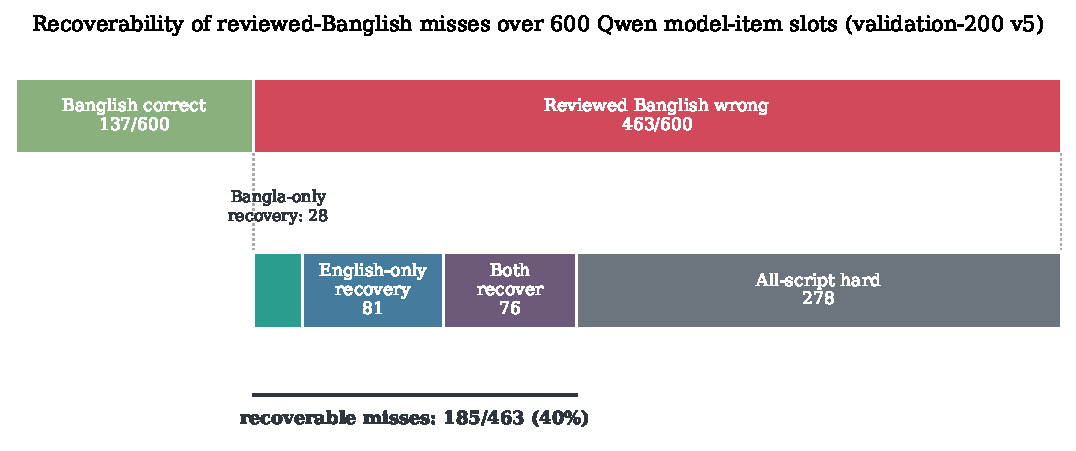
\includegraphics[width=\textwidth]{figures/fig_recoverability.pdf}
\caption{Recoverability decomposition of reviewed-Banglish misses over the 600 Qwen model-item slots of validation-200 v5. Of 463 Banglish misses, 185 (40\%) are answerable by the same model when the same item is shown in Bangla or English.}
\label{fig:recoverability}
\end{figure}

This decomposition gives two important messages.

First, a large share of Banglish errors are not impossible items. In BEnQA, 55.2\% of Banglish misses are recoverable by Bangla or English. These are the clearest qualitative examples for the thesis: the same answer becomes reachable when the script view changes.

Second, the result is not absolute. Banglish-only success exists. There are 20/600 model-item slots where reviewed Banglish is correct and both alternate views are wrong. We therefore avoid saying ``Banglish is always worse.'' The claim is aggregate and paired: reviewed Banglish is systematically less reliable for the models and tasks studied.

\begin{table}[H]
\centering
\caption{Example recoverable reviewed-Banglish misses from the BEnQA extension}
\label{tab:recoverable-examples}
\small
\resizebox{\textwidth}{!}{%
\begin{tabular}{llllll}
\hline
Model & ID & Gold & Correct script views & Parsed answers & Banglish prompt fragment \\
\hline
Qwen2.5-3B & \texttt{...0100} & C & Bangla, English & BN=C; BG=D; EN=C & \texttt{akotin o mayosin...} \\
Qwen2.5-3B & \texttt{...0120} & D & Bangla, English & BN=D; BG=B; EN=D & \texttt{byakoteriyate...} \\
DeepSeek V4 Flash & \texttt{...0001} & C & Bangla, English & BN=C; BG=B; EN=C & \texttt{salokosongshleshoner...} \\
DeepSeek V4 Flash & \texttt{...0023} & A & Bangla & BN=A; BG=D; EN=D & \texttt{kshariy mutr...} \\
\hline
\end{tabular}%
}

\smallskip
{\footnotesize \texttt{BN}, \texttt{BG}, and \texttt{EN} denote parsed answers under Bangla, reviewed Banglish, and English prompts.}
\end{table}

These examples should not be read as a separate test. They are explanatory evidence. They show the mechanism of the paired result: the same item and answer can become unreliable when the input is written in reviewed Banglish.

\section{Error Taxonomy: Why Banglish Fails}

The recoverability counts say that failures are not random difficulty, but they do not say what goes wrong. To answer the ``but why does it fail?'' question, we code every one of the 164 recoverable BEnQA reviewed-Banglish misses across the three Qwen models into four categories using documented deterministic rules (\path{scripts/analyze_banglish_error_taxonomy.py}). Because these are recoverable misses, the model demonstrably can answer the item in Bangla or English, so each category isolates a failure introduced by the romanization itself rather than item difficulty.

\begin{table}[H]
\centering
\caption{Error taxonomy of the 164 recoverable BEnQA reviewed-Banglish misses across the three Qwen models.}
\label{tab:error-taxonomy}
\small
\begin{tabular}{lrr}
\hline
Category & Count & Share \\
\hline
Named-entity / technical-term corruption & 58 & 35.4\% \\
Number / unit / formula misread & 53 & 32.3\% \\
Romanized-word ambiguity & 51 & 31.1\% \\
Option-format failure & 2 & 1.2\% \\
\hline
Total & 164 & 100\% \\
\hline
\end{tabular}%
\end{table}

The categories are nearly balanced, which is itself informative: there is no single dominant failure mode, so a narrow fix will not close the gap.

\textbf{Named-entity / technical-term corruption (35\%)} is the largest category. The decisive options are romanized scientific terms whose Bangla spelling encodes a precise concept. In \texttt{benqa\_10th-Biology\_0128} the options are \texttt{lyakotik esid}, \texttt{glukoj}, \texttt{oksalo asitik esid}, and \texttt{glisarik esid} (lactic acid, glucose, oxaloacetic acid, glyceric acid); Qwen2.5-3B answers correctly in Bangla and English but selects the wrong romanized term. The romanization is faithful, but the model fails to ground the Latin-script chemistry vocabulary back to the concept.

\textbf{Number / unit / formula misread (32\%)} covers items that hinge on digits, units, or chemical formulae embedded in romanized text. In \texttt{benqa\_10th-Biology\_0215} the stem carries the glycolysis formula \texttt{C\_\{6\}H\_\{12\}O\_\{6\} $\rightarrow$ C\_\{3\}H\_\{4\}O\_\{3\}} alongside a romanized Roman-numeral option list; the model recovers the item in English but mis-selects under Banglish, where the mixed numeric-plus-romanized context is harder to parse.

\textbf{Romanized-word ambiguity (31\%)} is the residual category where ordinary Bangla words become ambiguous in Latin script and shift the model toward a wrong but plausible option. \texttt{benqa\_10th-Physics\_0280} asks for copper's resistivity (\texttt{tamar rodhokotto}); the numeric options differ only at the second significant figure, and the model picks the wrong value under Banglish while answering correctly in English.

\textbf{Option-format failure (1\%)} is rare here: only two recoverable misses produce an unparseable answer. The reviewed Banglish field almost always yields a clean A--D letter, so the gap is overwhelmingly about choosing the wrong option, not about violating the answer contract --- which rules out a trivial parsing explanation. Full per-item codings are in \path{reports/banglish_error_taxonomy.md}.

\endinput
